% !TeX program = pdflatex

\documentclass[11pt, math=mtpro2, color=blue, lang=en, mode=fancy]{CLS/elegantbookr}

% \documentclass[11pt, math=mtpro2, color=blue, lang=en]{elegantbook}


\usepackage{CLS/wb4ca}
\usepackage{longtable}

\geometry{
	letterpaper,
	top=0.9in,
	bottom=0.8in,
	left=0.8in,
	right=0.8in,
	% footsep=0pt
	}



\fancyheadoffset[LO,LE]{0cm}

	
\setlength\columnsep{10pt}
\setlength{\footskip}{6pt}
\setlength{\parindent}{0pt}
\setlength{\parskip}{0pt plus 1pt minus 1pt}
\setlength{\parsep}{2pt plus 1pt minus 1pt}
\setlength{\topsep}{2pt plus 1pt minus 1pt}
\setlength{\multicolsep}{1pt plus 1pt minus 1pt}

\def\rotationdegree{180}

\raggedcolumns % to align multicols by top.


\begin{document}

% \maketitle

% !TEX root=../MA119-Main.tex

\begin{titlepage}
	\thispagestyle{empty}%

	\begin{center}
		\setstretch{2.5}
		\bfseries
		\vspace*{2\baselineskip}
		{\Huge\raggedright \color{main} A Concise Workbook for College Algebra \par}
		\hrulefill\par
		{\LARGE\raggedleft \color{third}{Fei Ye}\par}%
	\end{center}%
	\vspace*{10\baselineskip}
	\vfill
	\color{second}
	\begin{center}
		{
		\large\color{second}
		Department of Mathematics and Computer Science\\[1ex]
		Queensborough Community College - CUNY\\[3ex]
		}

		{\cyan
		\today \\[1ex]
		 Version 2.0
		}
	\end{center}

	\vspace*{1\baselineskip}

	\end{titlepage}


	\frontmatter
	\thispagestyle{empty}
	
	\vspace*{2\baselineskip}
	
	
	\begin{flushleft}
		Dr. Fei Ye\\
		Department of Mathematics and Computer Science\\
		Queensborough Community College of CUNY\\
		222-05 56th Street, Bayside, NY, 11364\\
		email: feye@qcc.cuny.edu
	
		\null\vfill
	
		\textit{A Concise Workbook for College Algebra}
	
		\bigskip
	
		\textcopyright 2019 
		Fei Ye
	
		\bigskip
	
	
	
		% \textbf{Creative Commons License}.\\[0.25em]
	
		\includegraphics{pics/by-nc-sa.eps}
	
		This work is licensed under a Creative Commons
		\href{https://creativecommons.org/licenses/by-nc-sa/4.0/}{\blue{Attribution-NonCommercial-ShareAlike 4.0 International License}}.
	
	\end{flushleft}

% \newpage

% \frontmatter

% !TEX root=../MA119-Main.tex

\chapter*{Preface to the First Edition}
% \addcontentsline{toc}{chapter}{Preface} 
\markboth{Preface}{} 

This workbook mainly grew out of the author's worksheets for the college algebra course (MAD-119) at QCC of CUNY.
It is intended to give a concise introduction to College Algebra.
  

In teaching College Algebra, I feel strongly that instructors should emphasize more the depth of reasoning and understanding rather than multitudes of approaches to similar types of questions. If you think carefully, whenever you choose an approach to solve a  problem, there is always a reason. Students should learn why an approach works instead of simply following the procedure which in nowadays can be done by computers. 

Motivated by the above thought, in this concise workbook, we try to expose only key concepts and ideas, which will save time for practicing and
reinforcing critical thinking skills which include observing patterns, identifying and analyzing problems, making logic connections, determining problem-solving strategies, and solving problems systematically.

For example, only the method of undetermined coefficient was introduced for factoring trinomials in this book. To factor the trinomial $Ax^2+Bx+C$, where $A$, $B$ and $C$ are integers, we may use trial-and-error method to find integers $m$, $n$, $p$ and $q$ such that $mn=A$, $pq=C$ and $mq+np=B$.
In practice, we first factor $A$ and $C$, and then use the following diagram to check if $mq+np=B$ holds.
\begin{center}
	\begin{tikzpicture}
		\matrix (m) [
			matrix of math nodes,
			row sep=-\pgflinewidth,
			column sep=-.5\pgflinewidth,
			minimum width=2em,
		]
		{ A=mn                  & {} & C=pq &                        \\[0.5em]
			m                     & {} & p    &                        \\
			n                     & {} & q    &                        \\[0.25em]
			\overset{\phantom{?}}{np} & {\color{red} +} & mq   & \overset{?}{=}B \\
		};
		\path
		(m-2-1) edge (m-3-3)
		(m-2-3) edge (m-3-1);
		\draw[red] (m-4-1.north west) -- (m-4-4.north east);
	\end{tikzpicture}
\end{center}
This method is based on the observation that $Ax^2+Bx+C$ can be factored into $(mx+p)(nx+q)$.
Indeed, observing and making logic connections are very effective in problem-solving.


Topics are contained in 25 lessons.  Each lesson corresponds to roughly one class meeting. A lesson starts with a page on concepts, formulas and examples, and ends with exercises that students are expected to complete in class.

We would like to thank our colleagues and students for their feedback and support during the development of this project.
In particular, we would like to thank 
Joseph Bertorelli,
Beata Ewa Carvajal,
Kwai Chiu,
Lixu Li,
Wenjian Liu,
Nam Jong Moh,
Tian Ren,
Kostas Stroumbakis,
Evelyn Tam,
and
Haishen Yao
for their encouragement, support, and feedback.


% \vspace*{\baselineskip}
\begin{flushright}
	\parbox{\lengthsignature}{
		Fei Ye\\
		Fall 2018
	}
\end{flushright}

\let\clearpage\relax

\vspace*{1.5\baselineskip}

\chapter*{Preface to the Second Edition}
% \addcontentsline{toc}{chapter}{Preface} 
\markboth{Preface}{} 


Effective practice is the key for success. Focusing on key ideas, frequently used problem solving strategies and necessary knowledge is the best way to practice effectively.

In this second edition, more examples and exercises are provided. Some frequently used problem solving strategies and ideas are summarized as tips.

In algebra, problem solving is meaningful, for each step you take, there is always a reason. I hope that you will agree with me and enjoy thinking and understanding the powerful ideas hidden in algebraic problem solving.


% \vspace*{\baselineskip}
\begin{flushright}
	\parbox{\lengthsignature}{
		Fei Ye\\
		Fall 2019
	}
\end{flushright}

\renewcommand{\baselinestretch}{1.0}\normalsize


\newpage

\blankpage

% \input{frontmatter/preface2.tex}

% \newpage

% \blankpage

% !TEX root=../MA119-Main.tex

\renewcommand{\baselinestretch}{0.975}
% \normalsize

\tableofcontents

\clearpage
\thispagestyle{empty}
\mainmatter
\hypersetup{pageanchor=true}
\newpage
\thispagestyle{empty}
\newpage

\blankpage

\mainmatter

\renewcommand{\baselinestretch}{1.05}\normalsize

\chapter{Linear Inequalities}
\import{Lessons/}{MA119-05-Linear-Inequalities.tex}
\newpage


\chapter{Absolute Value Equations}
\import{Lessons/}{MA119-06-Absolute-Value-Eq.tex}
\newpage

% \blankpage

\chapter{Properties of Integral Exponents}
\import{Lessons/}{MA119-01-Exponents.tex}
\newpage

% \blankpage

\chapter{Introduction to Functions}
\import{Lessons/}{MA119-02-Introduction-Functions-and-Graphs.tex}
\newpage

% \blankpage

\chapter{Linear functions}
\import{Lessons/}{MA119-03-a-Linear-Functions.tex}
\newpage


\chapter{Perpendicular and Parallel Lines}
\import{Lessons/}{MA119-03c-More-Linear-Functions(Perp-Parallel).tex}
\newpage


\chapter{Systems of Linear Equations}
\import{Lessons/}{MA119-04-Linear-Systems.tex}
\newpage


\chapter{Factoring Review}
\import{Lessons/}{MA119-07-Factoring-Review.tex}
\newpage


\chapter{Solve Quadratic Equations by Factoring}
\import{Lessons/}{MA119-08-Quadratic-Equations-by-Factoring.tex}
\newpage

% \blankpage

\chapter{Multiply or Divide Rational Expressions}
\import{Lessons/}{MA119-09-Multiplying-Dividing-Rational-Expressions.tex}
\newpage

\chapter{Add or Subtract Rational Expressions}
\import{Lessons/}{MA119-10-Adding-Subtracting-Rational-Expressions.tex}
\newpage

\chapter{Complex Rational Expressions}
\import{Lessons/}{MA119-11-Complex-Rational-Expressions.tex}
\newpage


\chapter{Rational Equations}
\import{Lessons/}{MA119-12-Rational-Equations.tex}
\newpage


\chapter{Radical Expressions: Concepts and Properties}
\import{Lessons/}{Math119-13-Radical-Expressions-Rational-Exponents.tex}
\newpage


% \blankpage

\chapter{Algebra of Radicals}
\import{Lessons/}{Math119-16-Multiply-Add-Radicals.tex}
\newpage

%\blankpage

\chapter{Solve Radical Equations}
\import{Lessons/}{Math119-17-Solve-Radical-Equations.tex}
\newpage


\chapter{Complex Numbers}
\import{Lessons/}{Math119-18-Complex-Numbers.tex}
\newpage

\chapter{Complete the Square}
\import{Lessons/}{Math119-19-Completing-Square.tex}
\newpage


\chapter{Quadratic Formula}
\import{Lessons/}{Math119-20-Quadratic-formula.tex}
\newpage


\chapter{Quadratic Functions}
\import{Lessons/}{Math119-21-Graph-Quadratic.tex}
\newpage



\chapter{Rational and Radical Functions}
\import{Lessons/}{Math119-21half-Rational-Radical-functions.tex}
\newpage


\chapter{Exponential Functions}
\import{Lessons/}{Math119-23-Exponential-Functions.tex}
\newpage


\chapter{Logarithmic Functions}
\import{Lessons/}{Math119-25-Logarithmic-Functions.tex}
\newpage

\chapter{Properties of Logarithms}
\import{Lessons/}{Math119-26-Properties-of-Logarithms.tex}
\newpage

\chapter{Exponential and Logarithmic Equations}
\import{Lessons/}{Math119-28-Exponential-and-Logarithms-Equations.tex}
\newpage


\end{document}